\section{Runtime Inefficiencies}
\label{removal}

The identification and removal of inefficiencies follows the same iterative approach presented in section \ref{identification}.

\subsection{Multithreading Inefficiencies}

Without the sensibility provided by the tests in section \ref{identification}, a scientist would incur in the pitfall of using all available cores (and even all hardware threads) on the system, hoping that it would provide the best performance. While it may be true for the non-pointer implementation,the system computational resources would be used inefficiently, and using the single device highly efficient pointer implementation would induce a even greater waste.

A closer look to the pointer implementation is needed since it is the most efficient. As seen in section \ref{data_inef}, the scalability of the parallelization is restricted by the NUMA memory accesses required by the shared memory. If the threads on $cpu_1$ do not share information with the threads on $cpu_2$ the bottleneck is removed, which can be achieved by using multithreaded processes. An MPI paralllelization at the event level is impossible by the reasons referred in section \ref{data_inef}.

Analysis applications are executed individually for each file (around 1GB in size) in a huge set of files, usually reaching the terabyte scale, received from CERN each week. An alternative approach to the MPI parallelization is to balance the execution of different \tth processes in the system on a set of input files. This reduces the complexity of the implementation, with no changes needed for \tth, and avoids communication between processes. A simple scheduler was devised, which takes a set of input files and creates a given amount of \tth processes. It is then responsible for dispatching the files to the different processes in a queue-like approach, and monitor their execution, as shown in figure \ref{fig:sched_flow}. A set of 20 input files was considered for testing purposes, with different configurations of processes and threads per process.

\begin{figure}[!htp]
	\begin{center}
		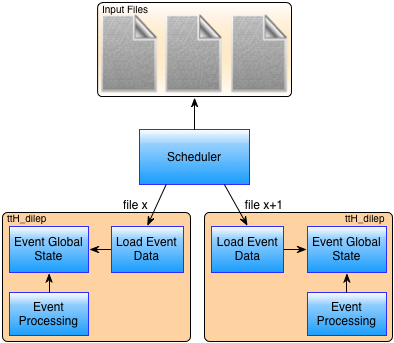
\includegraphics[scale=0.4]{images/scheduler_workflow.png}
		\caption{Schematic representation of dispatcher workflow.}
		\label{fig:sched_flow}
	\end{center}
\end{figure}

Figure \ref{fig:Sched} presents the speedups using 2, 4, 5, 8, and 10 processes for various thread configurations, with maximum number of threads was limited to 40. The best speedups occur for 8 processes with 5 threads each, with a peak of 55.6, 6 and 10 times better than the non-pointer and pointer implementations, respectively. A small number of threads such as this allows for a small overhead in the \tth parallelization, namely on load balancing and final best reconstruction merge for each event. A common behaviour is that when using the CPU devices hardware multithreading the speedups tend to stabilize, or even drop in the case of 2, 4, and 5 processes.

\begin{figure}[!htp]
	\begin{center}
		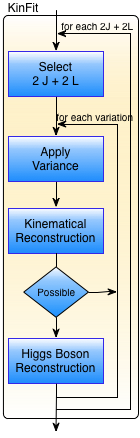
\includegraphics[scale=0.6]{images/sequential_kinfit.png}
		\caption{Speedups for the scheduler with 2, 4, 5, 8, and 10 processes with various thread configurations.}
		\label{fig:Sched}
	\end{center}
\end{figure}

\subsection{Core Affinity Inefficiencies}

The final possible optimization at runtime regards the thread affinity, i.e., control to which CPU cores a given thread is allocated. By default OpenMP allows for the Operating System to manage thread affinity, allowing for threads to be changed between cores during runtime. If a thread is running on core $c_1$ and it is moved to core $c_2$, all the data on the private cache $l_{c_1}$ needs to be reloaded to cache $l_{c_2}$, causing unnecessary overhead. This effect is amplified if the threads are moved between CPU devices. When multiple different, and possibly parallelized, processes are running on the same system, which is common in production environments, occurrences of bad scheduling occur more often.

Defining the thread affinity of an application may provide a more constant, or in some cases better, performance. In theory, an optimum thread affinity scheme allocates the threads to contiguous physical cores of one CPU device, uses the cores of the second CPU device only after the first is filled, and finally uses the multithreading after filling all physical cores. Note that using multithreading before the second CPU device may provide better performance in memory bound applications. This type of affinity must be defined prior to the application execution and depends on the system used. In this case the affinity was specifically tuned to this system for all threads, or process/threads configuration for the scheduler.

\begin{figure}[!htp]
	\begin{center}
		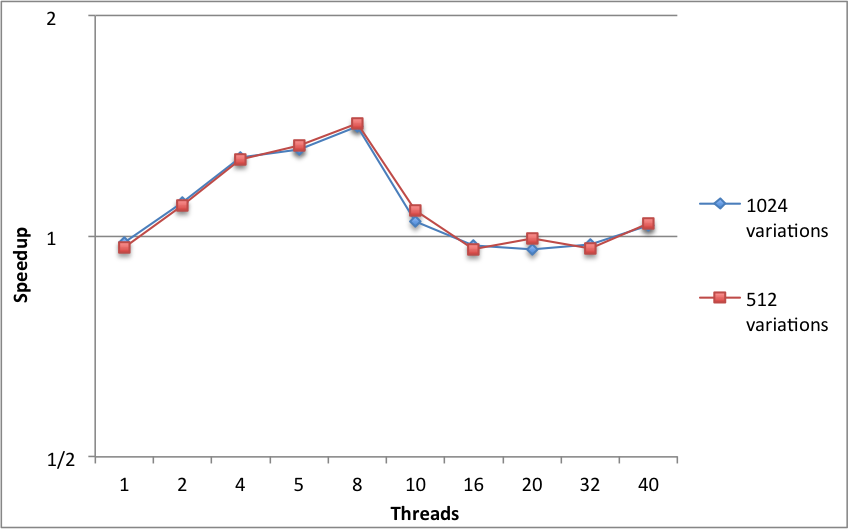
\includegraphics[scale=0.4]{charts/speedup_pointer_aff.png}
		\caption{Speedup of the \tth parallel pointer implementation with affinity \textit{vs} no affinity.}
		\label{fig:pointer_aff}
	\end{center}
\end{figure}

By analysing the speedups of the pointer implementation of \tth with thread affinity, in figure \ref{fig:pointer_aff}, it is concluded that specifying the affinity is provides speedups for the previous most efficient number of threads, i.e., up to 8 threads. For 8 threads the performance increases by 41\%, relative to its no affinity counterpart. With this number of threads, and the amount of shared data, moving threads between cores at runtime causes more cache warm ups to occur, significantly affecting the performance. When using more than 10 threads the application is roughly 4\% slower as the Operating System uses some multithreaded cores rather than using all available physical cores and it does a better job at managing the multithreading.

MELHORIA DE PERFORMANCE SCHEDULER

MELHORIA DE PERFORMANCE OVERALL
